\chapter{Marco metodológico}
\label{cap:metodologia}

El presente capítulo describe la estrategia metodológica empleada para el desarrollo del sistema propuesto, detallando las diferentes fases, enfoques y herramientas utilizadas. El enfoque metodológico adoptado se fundamenta en un híbrido entre dos paradigmas: el modelo en cascada, que es más tradicional y estructurado, y las prácticas ágiles, que permiten una mayor flexibilidad y retroalimentación temprana al utilizar un desarrollo incremental. 

Esta combinación se justifica por la naturaleza del proyecto, en condición de Trabajo Final de Graduación, que requiere un enfoque riguroso y extensamente documentado, con poco margen para cambios significativos en los requisitos una vez definidos, pero que también se beneficia de la iteración y la retroalimentación continua para asegurar que el sistema cumple con las expectativas del usuario final. 

A continuación, se describe con mayor detalle cada una de las etapas del proceso, así como un desglose de la correlación entre el marco metodológico y los objetivos específicos del proyecto, planteados en la sección \ref{secc:objectives}.


\section{Explicación del enfoque metodológico}

El modelo en cascada o \textit{waterfall}, descrito en \cite{royce_waterfall_1970}, se caracteriza principalmente por su enfoque secuencial, donde cada fase del desarrollo debe completarse antes de pasar a la siguiente. A grandes rasgos, un proceso de este tipo sigue las siguientes etapas:

\begin{enumerate}
    \item \textbf{Requerimientos:} En esta fase se recogen y documentan los requisitos del sistema, asegurando que se entienden las necesidades del cliente y los objetivos del proyecto.
    \item \textbf{Diseño:} Se elabora un diseño detallado del sistema, incluyendo la arquitectura, los componentes y las interfaces necesarias para cumplir con los requisitos establecidos.
    \item \textbf{Implementación:} En esta etapa se desarrollan los componentes del sistema según el diseño previamente definido, utilizando las herramientas y tecnologías adecuadas.
    \item \textbf{Verificación:} Se realizan pruebas para verificar que el sistema cumple con los requisitos especificados, asegurando su funcionalidad y calidad.
    \item \textbf{Mantenimiento:} Una vez que el sistema está en funcionamiento, se realizan ajustes y mejoras según sea necesario, abordando cualquier problema que surja durante su operación.
\end{enumerate}

A pesar de que este modelo no suele ser la primera opción para proyectos de hardware y software, para los cuales normalmente se prefiere un enfoque ágil, sigue siendo una metodología que presenta ventajas para proyectos con ciertas particularidades. Por ejemplo, en proyectos donde el alcance y los entregables están bien definidos desde el inicio, la estructura secuencial del modelo en cascada funciona bastante bien. Esta característica se alinea convenientemente con la naturaleza del Trabajo Final de Graduación, donde los objetivos y requisitos deben ser claros desde las primeras etapas del proyecto, y aunque es posible modificar el alcance, idealmente se busca evitar cambios significativos una vez que se ha comenzado el desarrollo.

Otra ventaja del modelo en cascada es su enfoque en la documentación exhaustiva, lo que facilita la comprensión del sistema por parte de todos los involucrados y proporciona una base sólida para futuras referencias. Esto es particularmente útil para proyectos académicos, en los que la documentación técnica y el registro de decisiones son esenciales para la evaluación y la validación del trabajo realizado. También, el modelo en cascada permite dar un seguimiento claro del progreso del proyecto, ya que cada fase debe completarse antes de avanzar a la siguiente, lo que puede facilitar la gestión del tiempo, el cual es limitado en este contexto. 

Ahora bien, algunos de los puntos débiles del modelo \textit{waterfall} que se buscaron mitigar con la incorporación de prácticas ágiles son la rigidez en la adaptación a cambios y la falta de retroalimentación continua. En la metodología híbrida utilizada, se pretendió aplicar algunos de los 12 principios del Manifiesto Ágil, principalmente los siguientes:

\begin{enumerate}
    \item \textit{``Nuestra mayor prioridad es satisfacer al cliente mediante la entrega temprana y continua de software valioso \cite{agile_principles}.''} 
    \item \textit{``Los cambios en los requisitos son bienvenidos, incluso en las etapas tardías del desarrollo. Los procesos ágiles aprovechan el cambio para proporcionar ventaja competitiva al cliente \cite{agile_principles}.''}
\end{enumerate}

Se incorporaron estos dos principios en la \textbf{fase de implementación} del modelo en cascada mediante iteraciones cortas y revisiones frecuentes del sistema desarrollado. Esto implicó que se siguieran las etapas secuenciales de captura de requerimientos y diseño de alto nivel de la solución; sin embargo, durante la etapa de implementación, se realizaron ciclos cortos de planificación, diseño más preciso de cada módulo, desarrollo de las tareas comprometidas y procesos de verificación. Esto con la intención de que con base en la retroalimentación de la contraparte de la organización, fuera posible hacer ajustes y mejoras necesarias, pero que no afectaran significativamente el alcance del proyecto. 

Posteriormente, se procede con la fase de verificación, donde se evalúa el sistema en su totalidad con pruebas de punto a punto, para las cuales se esperaba un alto grado de éxito, dado que se realizaron pruebas parciales durante la fase de implementación. La etapa de mantenimiento quedó fuera del alcance de este proyecto en su calidad de Trabajo Final de Graduación debido a las restricciones de tiempo, sin embargo, el sistema quedará integrado en la infraestructura de Fito App, por lo tanto, en su condición de producto comercial, será objeto de mantenimiento y mejoras continuas por parte del equipo de desarrollo de la organización.

En la Figura \ref{fig:metodologia} se presenta un diagrama que ilustra el enfoque metodológico adoptado, destacando las fases del modelo en cascada y la integración de prácticas ágiles durante la fase de implementación.

\begin{figure}[H]
    \centering
    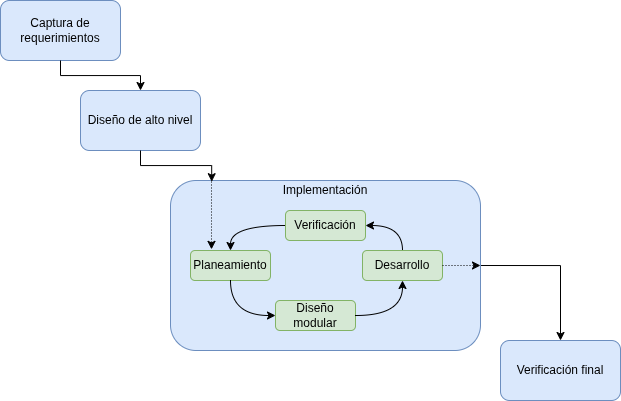
\includegraphics[width=0.8\textwidth]{methodology.png}
    \caption{Proceso metodológico adoptado para el desarrollo del sistema propuesto.}
    \label{fig:metodologia}
\end{figure}

Algunos puntos importantes a considerar en la implementación de este enfoque metodológico son:
\begin{itemize}
    \item Los ciclos de implementación tuvieron una duración de dos semanas.
    \item Cada ciclo incluyó una reunión de planificación con la contraparte de la organización, donde se definió el alcance y las tareas a realizar.
    \item Cada ciclo incluyó una etapa de diseño específica para cada módulo a desarrollar, pero que partió del diseño de alto nivel previamente establecido.
    \item Se mantuvo un tablero virtual al estilo Kanban para el seguimiento del estado de las tareas y el progreso del proyecto.
    \item Al final de cada ciclo se hizo una revisión del trabajo realizado con la contraparte organizacional, las cuales tomaron forma de pruebas de aceptación de usuario o demostraciones del sistema.
    \item En las sesiones de verificación se obtuvo retroalimentación continua, lo que permitió realizar ajustes y mejoras que se reflejaron en los ciclos siguientes.
\end{itemize}

\section{Actividades desarrolladas para cada objetivo específico del proyecto}

En la Tabla \ref{tab:activities} se presenta un desglose de las actividades realizadas para cada uno de los objetivos específicos planteados en la sección \ref{secc:objectives}, junto con sus entregables asociados, técnicas o herramientas utilizadas y estrategias de verificación implementadas. Para mayor facilidad de lectura, se utiliza el identificador de cada objetivo específico:

\objectives

Los entregables asociados a cada objetivo específico se pueden consultar en la Tabla \ref{tab:deliverables}, donde se añadió una breve descripción de cada entregable. Ahora bien, a continuación se enumeran dichos entregables con su respectivo identificador único que será referenciado en la tabla:

\begin{itemize}
    \item \textbf{E1:} \deliverablearch
    \item \textbf{E2:} \deliverabledet
    \item \textbf{E3:} \deliverableos
    \item \textbf{E4:} \deliverablerec
    \item \textbf{E5:} \deliverablerep
    \item \textbf{E6:} \deliverableperf
\end{itemize}

El listado de actividades desarrolladas para alcanzar el cumplimiento de los objetivos específicos del proyecto se presenta a continuación. Cada actividad también está asociada a un identificador único que se utiliza en la tabla para facilitar su referencia:

\begin{itemize}
    \item \textbf{A1-1:} Levantamiento de requisitos del sistema.
    \item \textbf{A1-2:} Selección comparativa de la plataforma de hardware.
    \item \textbf{A1-3:} Diseño de arquitectura física del hardware: mapeo de pines y buses de comunicación.
    \item \textbf{A1-4:} Diseño de arquitectura lógica del sistema.
    \item \textbf{A2-1:} Modelado de la experiencia de usuario y guion de pantallas.
    \item \textbf{A2-2:} Desarrollo del módulo de detección facial en nodo \textit{on-edge}.
    \item \textbf{A2-3:} Integración del módulo de detección facial con la interfaz de usuario.
    \item \textbf{A2-4:} Configuración de Yocto Project y generación de la primera imagen mínima.
    \item \textbf{A2-5:} Personalización de la imagen.
    \item \textbf{A2-6:} Adaptación de base de datos para el registro de accesos.
    \item \textbf{A2-7:} Habilitación de repositorio para almacenamiento de imágenes de los rostros de los usuarios.
    \item \textbf{A2-8:} Desarrollo de servicio \textit{serverless} para el registro de usuarios.
    \item \textbf{A2-9:} Desarrollo de servicio \textit{serverless} para el reconocimiento de usuarios y validación de membresía.
    \item \textbf{A2-10:} Publicación de \textit{endpoints} para utilizar los servicios.
    \item \textbf{A3-1:} Especificación de requisitos de información de reportes de acceso.
    \item \textbf{A3-2:} Implementación de servicios REST para el consumo de reportes de acceso.
    \item \textbf{A3-3:} Desarrollo de la interfaz de usuario para la visualización de reportes.
    \item \textbf{A4-1:} Elaboración del plan de pruebas.
    \item \textbf{A4-2:} Preparación del entorno de pruebas en gimnasio piloto.
    \item \textbf{A4-3:} Ejecución de pruebas de punto a punto del sistema.
    \item \textbf{A4-4:} Análisis estadístico de resultados y comparación con los objetivos de desempeño.
\end{itemize}


\begin{landscape} % Start landscape mode
    \begin{longtable}{l|l|p{2.5cm}|p{7cm}|p{7cm}}
        \caption{Desglose de actividades desarrolladas para cada objetivo específico.} \label{tab:activities} \\
        \hline
        \multicolumn{1}{c|}{\textbf{Obj. Esp.}} & \multicolumn{1}{c|}{\textbf{Entregables}} & \multicolumn{1}{c|}{\textbf{Actividades}} & \multicolumn{1}{c|}{\textbf{Herramientas/Técnicas}} & \multicolumn{1}{c}{\textbf{Estrategias de verificación}} \\ \hline
        \endfirsthead

        \multicolumn{5}{c}{\tablename \thetable{}: Desglose de actividades desarrolladas para cada objetivo específico (continuación).} \\
        \hline

        \multicolumn{1}{c|}{\textbf{Obj. Esp.}} & \multicolumn{1}{c|}{\textbf{Entregables}} & \multicolumn{1}{c|}{\textbf{Actividades}} & \multicolumn{1}{c|}{\textbf{Herramientas/Técnicas}} & \multicolumn{1}{c}{\textbf{Estrategias de verificación}} \\ \hline
        \endhead

        \hline
        \multicolumn{5}{r}{\textit{Continúa en la siguiente página}} \\ \hline
        \endfoot

        \hline
        \endlastfoot

        OE1 & E1 & A1-1, A1-2, A1-3, A1-4 & \vspace{-\baselineskip}
        \setlength{\leftmargini}{1em}
        \begin{itemize}
            \item Entrevistas con partes interesadas para el levantamiento de requisitos.
            \item Revisión de hoja de datos de Raspberry Pi 4B (plataforma disponible en la organización) y de sus posibles alternativas.
            \item Revisión de hoja de datos de cámaras compatibles.
            \item Revisión de hoja de datos de pantalla táctil compatible.
            \item Uso de software Draw.io para diagramas de arquitectura.
        \end{itemize} & \vspace{-\baselineskip}
        \setlength{\leftmargini}{1em}
        \begin{itemize}
            \item Aprobación de los requisitos del sistema por parte de la contraparte de la organización.
            \item Aprobación del documento de arquitectura física y lógica del sistema por parte de la contraparte de la organización.
            \item Verificación que el costo total de la plataforma de hardware no excede los \$300 USD.
        \end{itemize} \\
        \hline

        OE2 & E2, E3, E4 & A2-1, A2-2, A2-3, A2-4, A2-5, A2-6, A2-7, A2-8, A2-9, A2-10 & \vspace{-\baselineskip}
        \setlength{\leftmargini}{1em}
        \begin{itemize}
            \item Generación bosquejo (\textit{mockup}) de interfaz gráfica de usuario usando \textit{Draw.io}.
            \item Uso de \textit{git} para el control de versiones del código fuente. 
            \item Implementación de detección facial con \textit{C++} y \textit{OpenCV}.
            \item Generación de imagen Linux reproducible con \textit{poky} (Yocto).
            \item Orquestación de \textit{builds} con \textit{BitBake} (Yocto).
            \item Activación de capas como \textit{meta-yocto-bsp}, \textit{meta-poky} y \textit{meta-raspberrypi} para definir la plataforma y distribución (Yocto).
            \item Generación de SDK para permitir el desarrollo de aplicaciones sobre la imagen (Yocto).
            \item Creación o modificación de \textit{recipes} y archivos \textit{append} para incluir dependencias y configuraciones específicas (Yocto).
            \item Configuración de caché de estado para acelerar el proceso de compilación mediante el uso de \textit{sstate-cache} (Yocto).
        \end{itemize} & \vspace{-\baselineskip}
        \setlength{\leftmargini}{1em}
        \begin{itemize}
            \item Pruebas de usabilidad con los bosquejos de interfaz gráfica de usuario.
            \item Prueba de despliegue de la imagen Yocto en la Raspberry Pi 4B.
            \item Pruebas unitarias del módulo de detección facial que validan tasa de detección superior al 95\% con un banco de imágenes de referencia.
            \item Pruebas de \textit{endpoints} de servicios REST con \textit{Postman} (tipos de solicitudes, códigos de error, esquema de respuesta).
            \item Pruebas de precisión (mayor al 95\%) y latencia (menor a 500 ms) del servicio  de reconocimiento facial con un banco de imágenes de referencia.
            \item Pruebas de carga y resiliencia: hasta 50 peticiones concurrentes, sin degradación significativa de latencia ni errores 5XX.
            \item Validación de registros de acceso en la base de datos de Fito App.
        \end{itemize}\\
        \hline
        
         & & & \vspace{-\baselineskip}
        \setlength{\leftmargini}{1em}
        \begin{itemize}
            \item Uso de \textit{PostreSQL} para la modificación de la base de datos de Fito App y su adaptación a los requerimientos del sistema.
            \item Configuración de un \textit{bucket} en \textit{Amazon S3} para el almacenamiento de imágenes de rostros.
            \item Configuración de Red de Distribución de Contenidos (\textit{CDN}) para el consumo y distribución de imágenes.
            \item Uso de \textit{AWS Lambda} para el desarrollo de servicios \textit{serverless}.
            \item Uso de \textit{API Gateway} para la creación de \textit{endpoints REST}.
            \item Uso de API de \textit{Amazon Rekognition} para el reconocimiento facial.
            \item Uso de \textit{Python} para el desarrollo de servicios \textit{serverless} y comunicación con APIs.
            
        \end{itemize} & \\
        \hline

        OE3 & E5 & A3-1, A3-2, A3-3 & \vspace{-\baselineskip}
        \setlength{\leftmargini}{1em}
        \begin{itemize} 
            \item Uso de \textit{Node.js}, \textit{Drizzle ORM} y \textit{Neon SDK} para el desarrollo de servicios REST.
            \item Implementación con \textit{React} y \textit{Next.js} para la interfaz de usuario.
        \end{itemize} & \vspace{-\baselineskip}
        \setlength{\leftmargini}{1em} 
        \begin{itemize}
            \item Pruebas de usabilidad de la interfaz de reportes con usuarios administradores para evaluar claridad de las gráficas, tablas y filtros.
            \item Validación de consistencia de datos: comparación de un subconjunto de estadísticas contra los registros de acceso en la base de datos garantizando una desviación menor al 1\%.
            % \item Comprobación de que la paginación y el filtrado por fecha/usuario funcionan correctamente en distintos navegadores y resoluciones.
        \end{itemize}\\
        \hline

        OE4 & E6 & A4-1, A4-2, A4-3, A4-4 & \vspace{-\baselineskip}
         \setlength{\leftmargini}{1em}
         \begin{itemize}
            \item Medición de métricas de latencia en el reconocimiento facial, mediante la librería \texttt{std::chrono} en \textit{C++}.
            \item Registro manual de tasas de aciertos y fallos en el reconocimiento facial.
            \item Implementación de pruebas de aceptación de usuario (\textit{UAT}) con usuarios reales del gimnasio piloto.
            \item Uso de librerías de análisis estadístico y visualización de datos como \textit{Matplotlib} y \textit{NumPy} en \textit{Python} para el análisis de resultados.
         \end{itemize}
        & \vspace{-\baselineskip}
         \setlength{\leftmargini}{1em}
         \begin{itemize}
            \item Revisión del documento de los resultados y análisis por parte de la contraparte de la organización. 
         \end{itemize}\\
        \hline

    \end{longtable}
\end{landscape} % End landscape mode


